\documentclass[10pt, aspectratio=169]{beamer}

\usetheme{Madrid}
\usecolortheme{default}
\setbeamertemplate{navigation symbols}{}
\setbeamertemplate{footline}{%
  \hfill\insertframenumber/\inserttotalframenumber\hspace*{4pt}\vspace{2pt}}

\usepackage{booktabs}
\usepackage{multirow}
\usepackage{graphicx}
\usepackage{xspace}
\usepackage{adjustbox}
\usepackage{tikz}
\usetikzlibrary{positioning, arrows.meta, fit, calc}
\usepackage{listings}
\lstset{
  language=Python, basicstyle=\ttfamily\fontsize{5.5}{7}\selectfont,
  keywordstyle=\color{blue!70!black}\bfseries,
  commentstyle=\color{green!50!black}\itshape,
  stringstyle=\color{red!60!black},
  showstringspaces=false, frame=none, xleftmargin=0pt,
}

\graphicspath{{../../figures/}{../../images_ppt/}}

\title{Mini Colossal-AI}
\subtitle{Distributed Parallelism Strategies from Scratch}
\date{}
\author{}
\institute{}

\begin{document}

% ======== TITLE ========
\begin{frame}[plain]
  \vfill
  \centering
  \begin{beamercolorbox}[sep=12pt,center,rounded=true,shadow=true]{title}
    {\Large\bfseries Mini Colossal-AI}\\[0.4em]
    {\normalsize Distributed Parallelism Strategies from Scratch}
  \end{beamercolorbox}

  \vspace{1.5em}
  \begin{tabular}{c@{\hspace{2.5em}}c}
    \textbf{Dinesh Chand} & \textbf{Goutham P} \\
    {\scriptsize\texttt{dineshchand@iisc.ac.in}} & {\scriptsize\texttt{gouthamp@iisc.ac.in}} \\[0.8em]
    \textbf{Meena Chidambaram} & \textbf{Nadhiya R S} \\
    {\scriptsize\texttt{meenac@iisc.ac.in}} & {\scriptsize\texttt{nadhiyar@iisc.ac.in}} \\
  \end{tabular}

  \vspace{1.2em}
  {\small MTech-AI, IISc Bangalore}
  \vfill
\end{frame}

% ==================================================================
% PROBLEM STATEMENT & MOTIVATION  (Nadhiya)
% ==================================================================

\begin{frame}{Problem Statement \& Motivation}
  \begin{itemize}
    \item Training modern LLMs (100M--billions of parameters) requires distributing computation across multiple GPUs
    \item Multiple parallelism strategies exist (DP, TP, PP, ZeRO) --- each with different communication patterns and memory trade-offs
    \item The right strategy depends on both the \textbf{hardware topology} and the \textbf{model architecture}
  \end{itemize}

  \vspace{0.6em}
  \textbf{What we did:}
  \begin{enumerate}
    \item Built all four strategies \textbf{from scratch} using \texttt{torch.distributed} primitives
    \item Composed them into hybrid configurations through a unified 3D plugin
    \item Studied how \textbf{interconnect speed} and \textbf{axis-to-link mapping} affect throughput
    \item Tested across \textbf{two architectures} (GPT-2 and T5) to isolate architectural effects
  \end{enumerate}
\end{frame}

% ==================================================================
% METHODOLOGY  (Goutham)
% ==================================================================

% --- Four Strategies ---
\begin{frame}{Methodology: Four Parallelism Strategies}
  \begin{columns}[T]
  \begin{column}{0.55\textwidth}
    \begin{enumerate}
      \item \textbf{Data Parallelism (DP)}\\
      Replicate model on every GPU, average gradients via all-reduce after backward pass

      \item \textbf{ZeRO Optimizer Sharding}\\
      Stage~1: partition optimizer states\\
      Stage~2: also partition gradients\\
      Cuts per-GPU memory by up to $N\times$

      \item \textbf{Tensor Parallelism (TP)}\\
      1D column/row split (Megatron-LM style)\\
      2 all-reduces per transformer block

      \item \textbf{Pipeline Parallelism (PP)}\\
      1F1B asynchronous schedule\\
      Only sends activations between adjacent stages
    \end{enumerate}
  \end{column}
  \begin{column}{0.42\textwidth}
    \centering
    \small
    \begin{tabular}{ll}
      \toprule
      \textbf{Axis} & \textbf{Communication} \\
      \midrule
      DP & All-reduce gradients \\
         & (once per step) \\
      \midrule
      TP & All-reduce partial sums \\
         & (every layer, 2$\times$) \\
      \midrule
      PP & Send/recv activations \\
         & (between neighbors) \\
      \bottomrule
    \end{tabular}

    \vspace{0.6em}
    All implemented using only\\
    \texttt{dist.send}, \texttt{dist.recv},\\
    \texttt{dist.all\_reduce},\\
    \texttt{dist.all\_gather}
  \end{column}
  \end{columns}
\end{frame}

% --- Unified 3D Plugin ---
\begin{frame}{Methodology: Unified 3D Hybrid Plugin}
  \begin{columns}[T]
  \begin{column}{0.55\textwidth}
    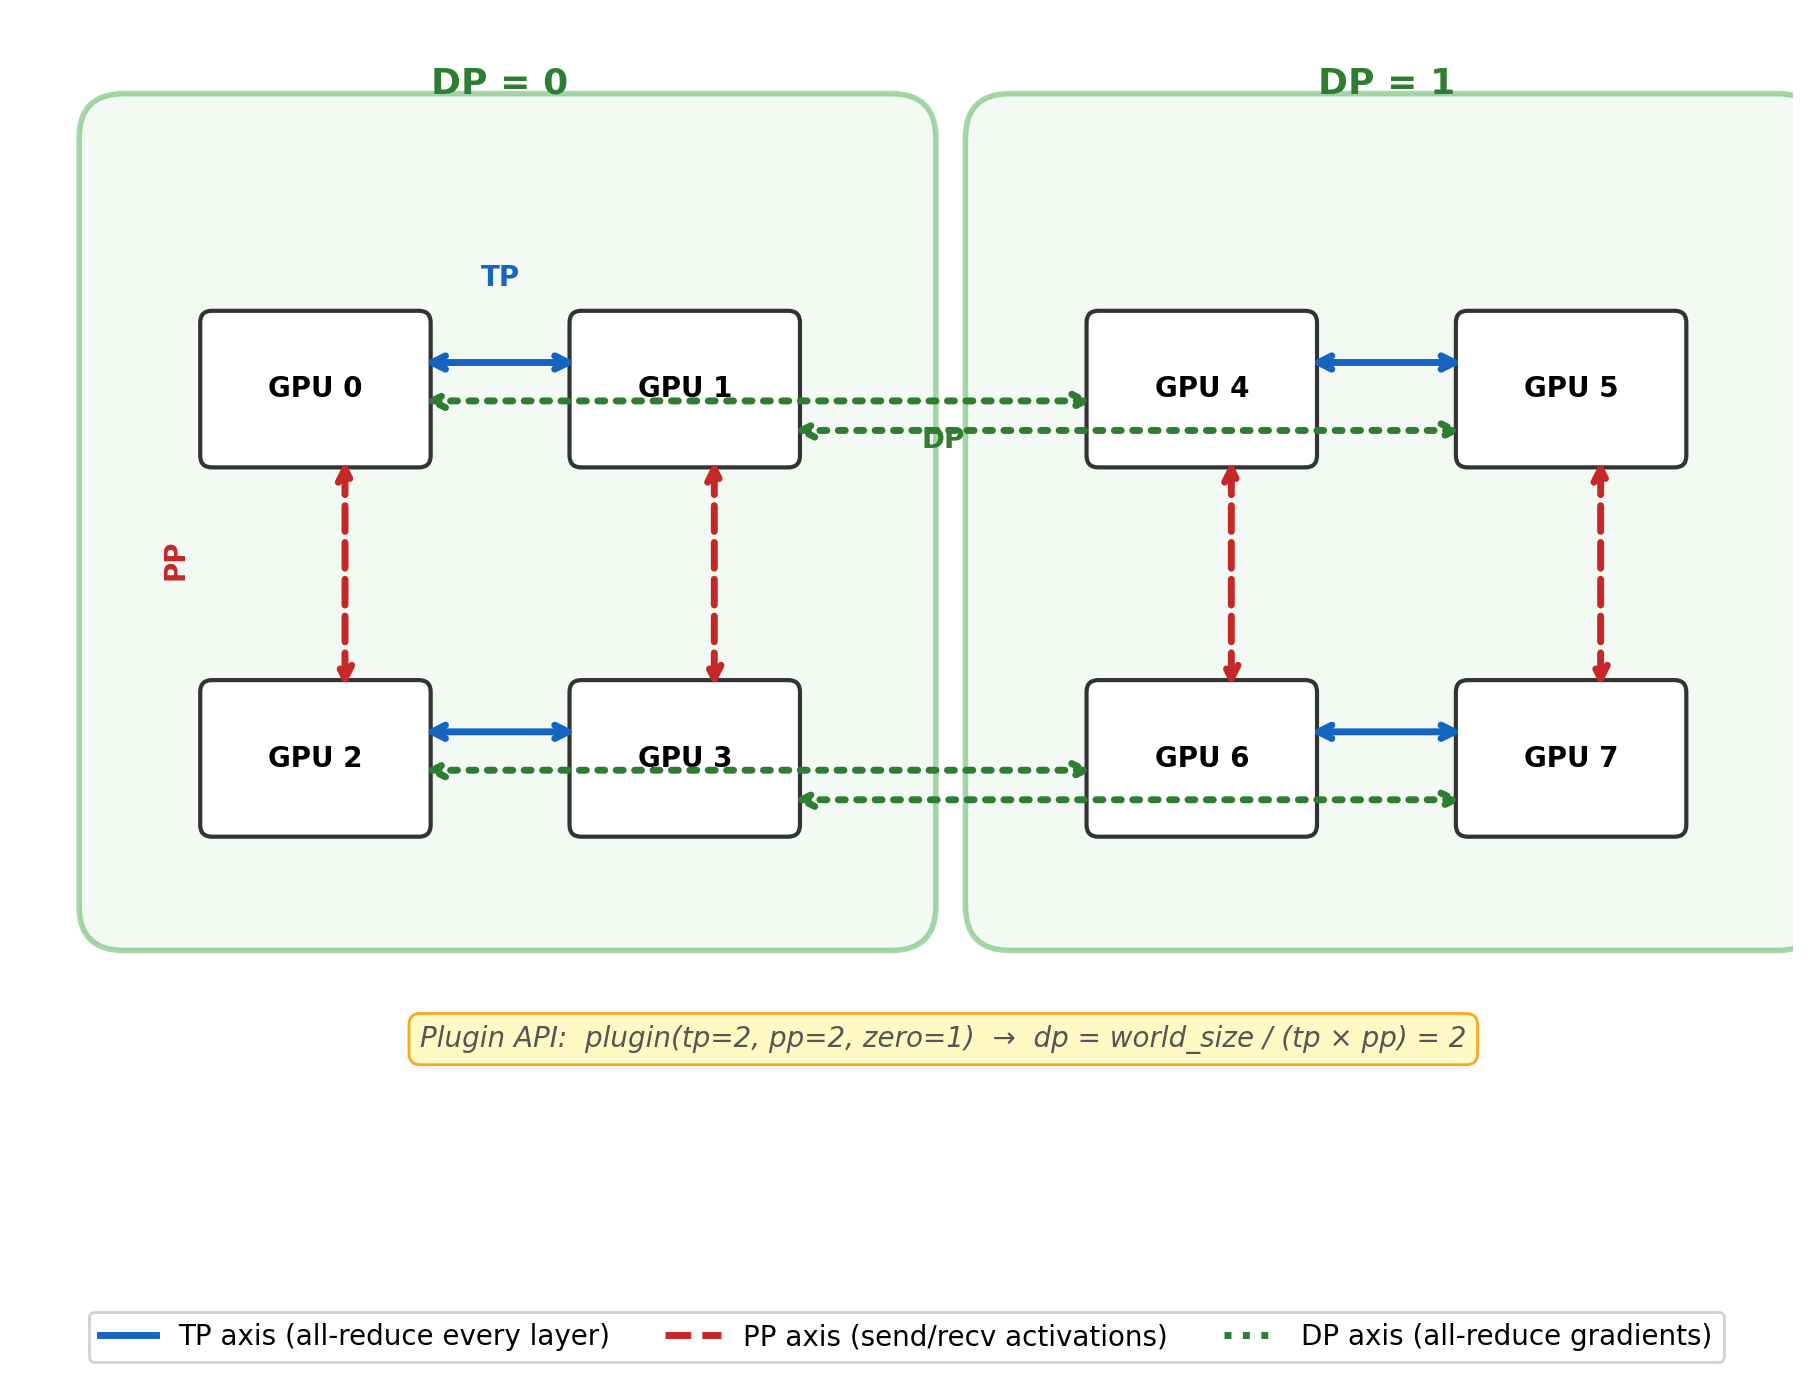
\includegraphics[width=\textwidth]{fig_ppt_3d_mesh.png}
  \end{column}
  \begin{column}{0.42\textwidth}
    \small
    One plugin handles all combinations:

    \vspace{0.3em}
    \texttt{plugin(tp=2, pp=2, zero=1)}\\
    $\rightarrow$ dp = world\_size / (tp $\times$ pp)

    \vspace{0.5em}
    \begin{itemize}
      \item Creates a 3D process group mesh
      \item Each GPU belongs to exactly one TP, PP, and DP sub-group
      \item All standalone components accept a process group argument
      \item No code duplication between standalone and hybrid modes
    \end{itemize}

    \vspace{0.3em}
    With 4 GPUs (Phase~2): 2 axes\\
    With 8 GPUs (Phase~3): all 3 axes
  \end{column}
  \end{columns}
\end{frame}

% --- How Placement Works (follows directly from the mesh) ---
\begin{frame}{How Placement Works: Reorder the Mesh Axes}
  \vspace{-0.8em}
  \centering
  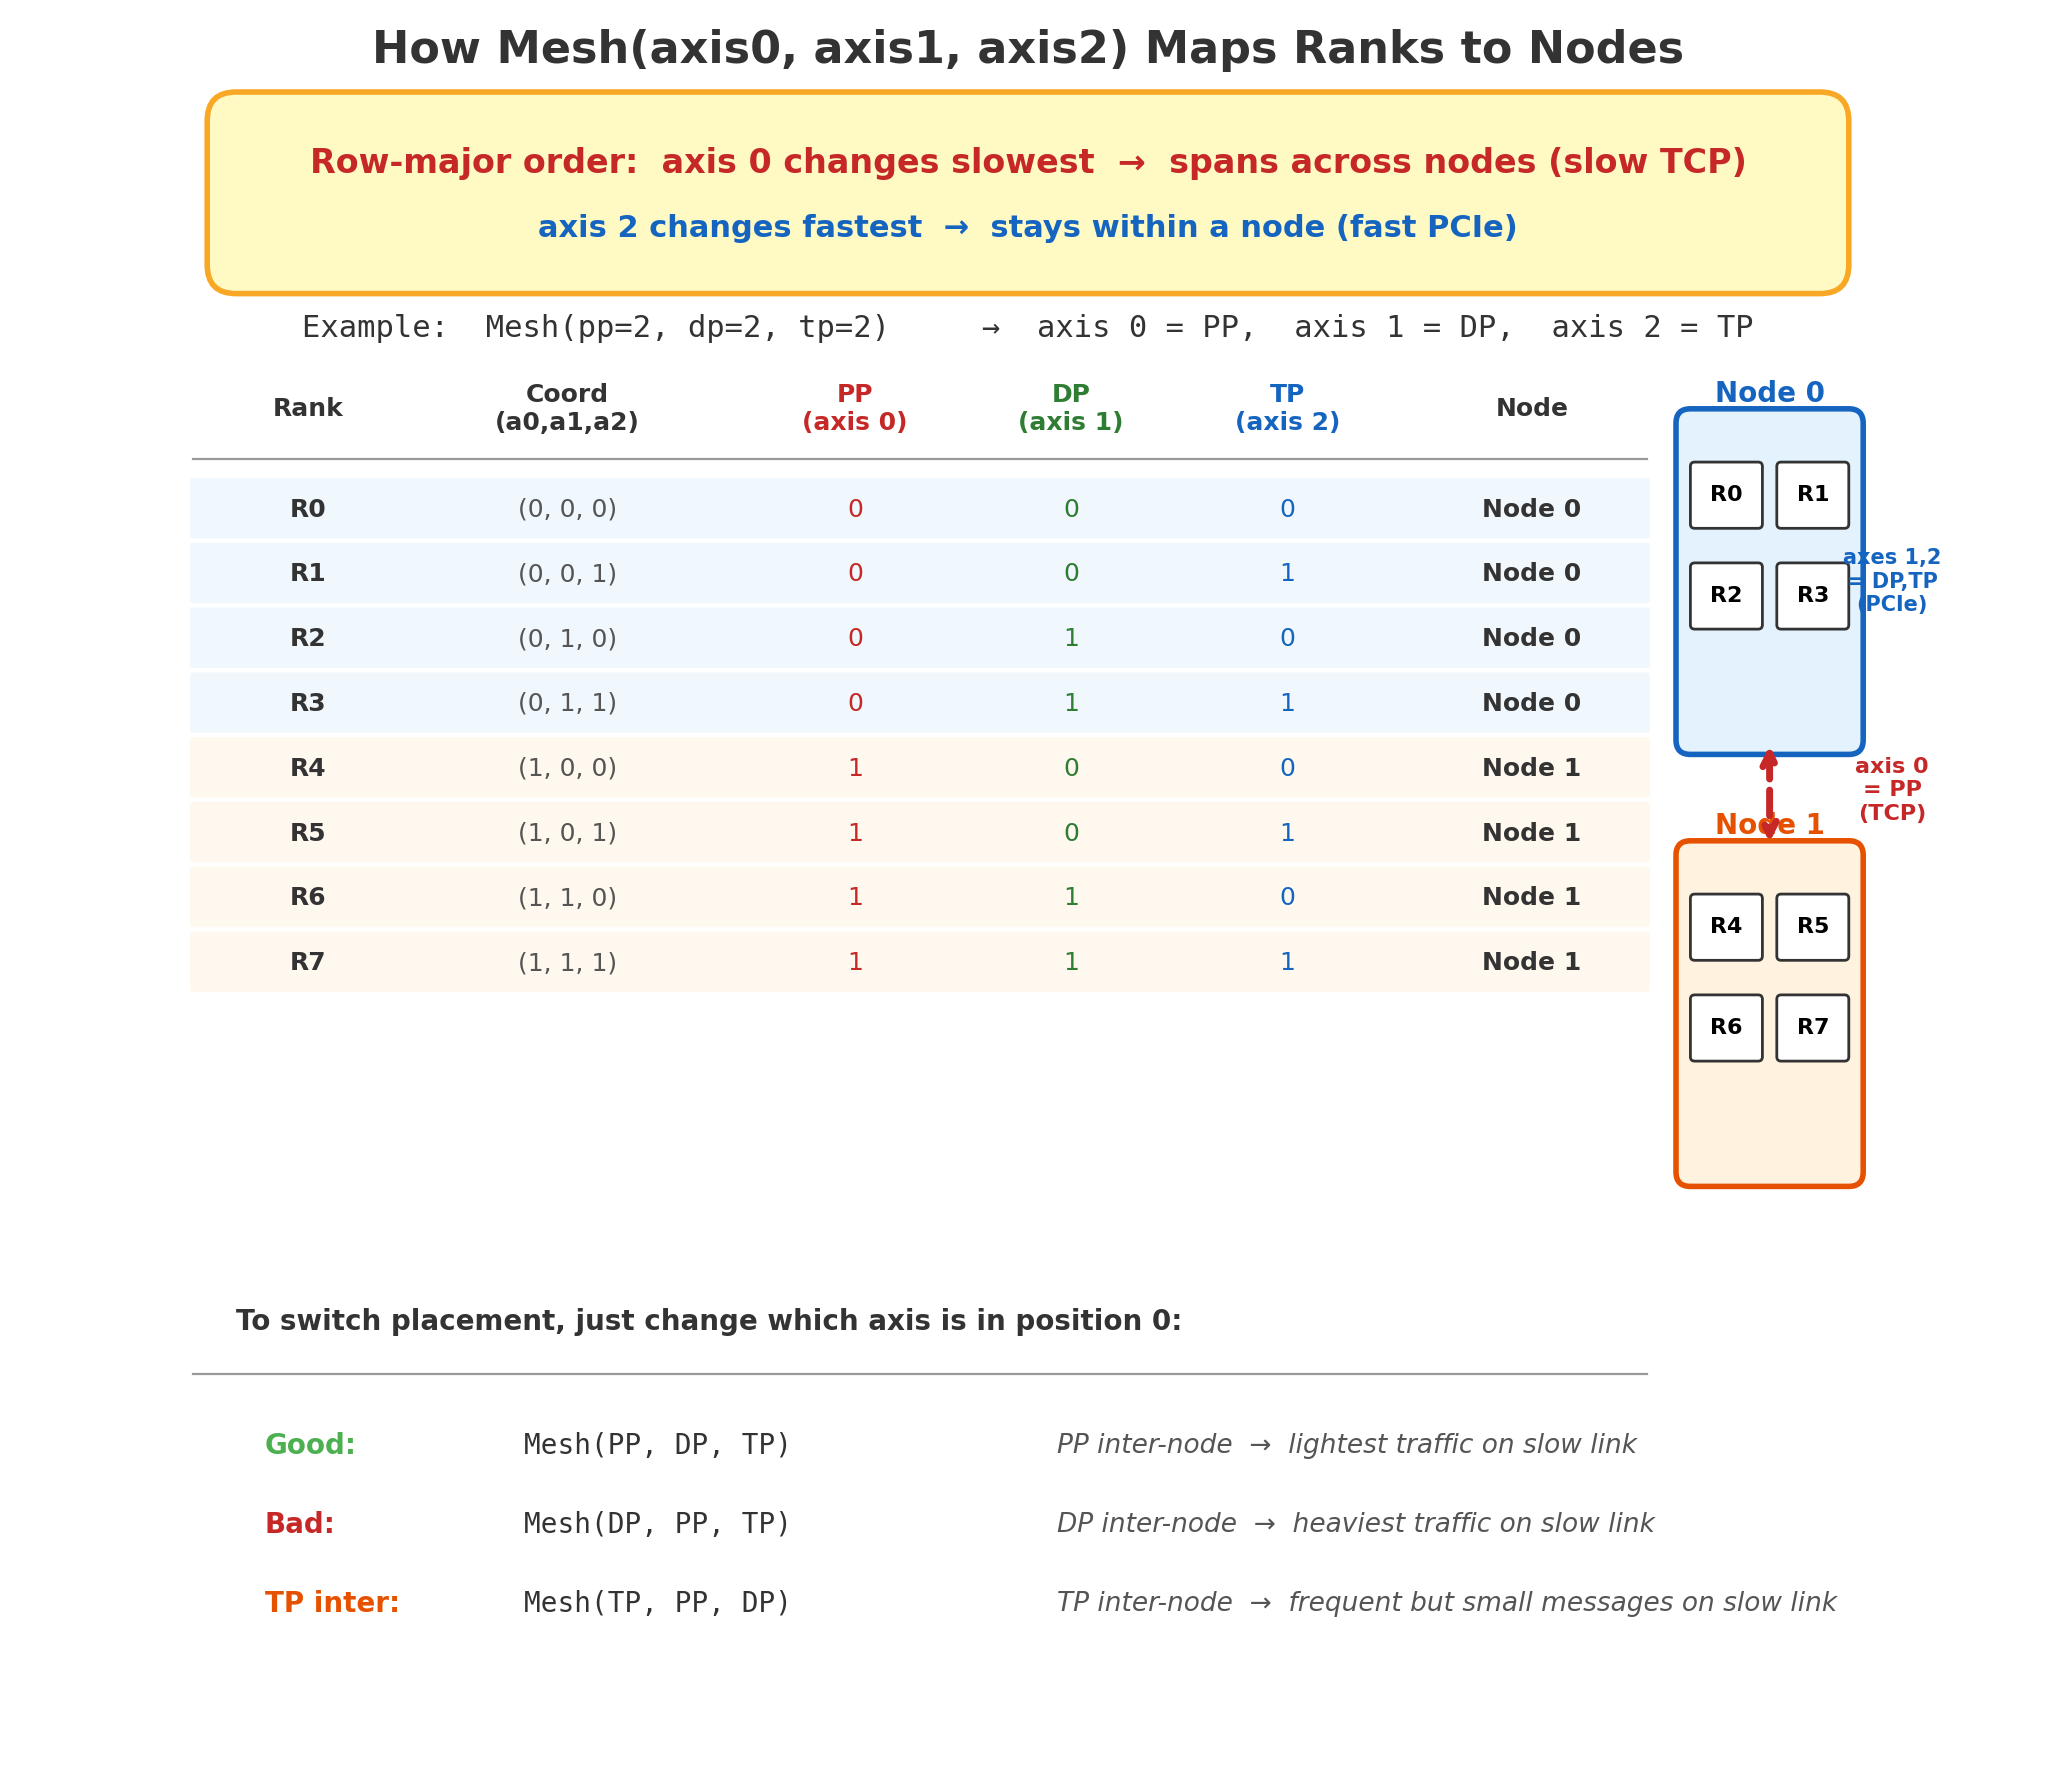
\includegraphics[height=0.85\textheight]{fig_ppt_axis_placement.png}
\end{frame}

% --- Hardware Setup ---
\begin{frame}{Methodology: Hardware Setup}
  \centering
  \adjustbox{max width=\textwidth}{%
  \begin{tabular}{lll}
    \toprule
    & \textbf{Phase 2: g4dn.xlarge} & \textbf{Phase 3: g4dn.12xlarge} \\
    \midrule
    \textbf{Nodes} & 4 instances & 2 instances \\
    \textbf{GPUs / node} & 1$\times$ T4 (16 GB) & 4$\times$ T4 (16 GB each) \\
    \textbf{Total GPUs} & 4 & 8 \\
    \textbf{Intra-node link} & N/A (single GPU per node) & PCIe ($\sim$15 GB/s) \\
    \textbf{Inter-node link} & TCP ($\sim$0.6 GB/s) & TCP ($\sim$0.6 GB/s) \\
    \bottomrule
  \end{tabular}}

  \vspace{1.0em}

  \begin{columns}[T]
  \begin{column}{0.48\textwidth}
    \centering
    \textbf{Phase 2:} Every GPU-to-GPU link is TCP\\
    $\Rightarrow$ All strategies share the same slow link
  \end{column}
  \begin{column}{0.48\textwidth}
    \centering
    \textbf{Phase 3:} \textbf{25$\times$ bandwidth gap}\\
    Fast PCIe within node, slow TCP between nodes\\
    $\Rightarrow$ Which axis goes where matters
  \end{column}
  \end{columns}
\end{frame}

% --- Communication-Aware Placement ---
\begin{frame}{Methodology: Communication-Aware Placement}
  \vspace{-0.3em}
  \centering
  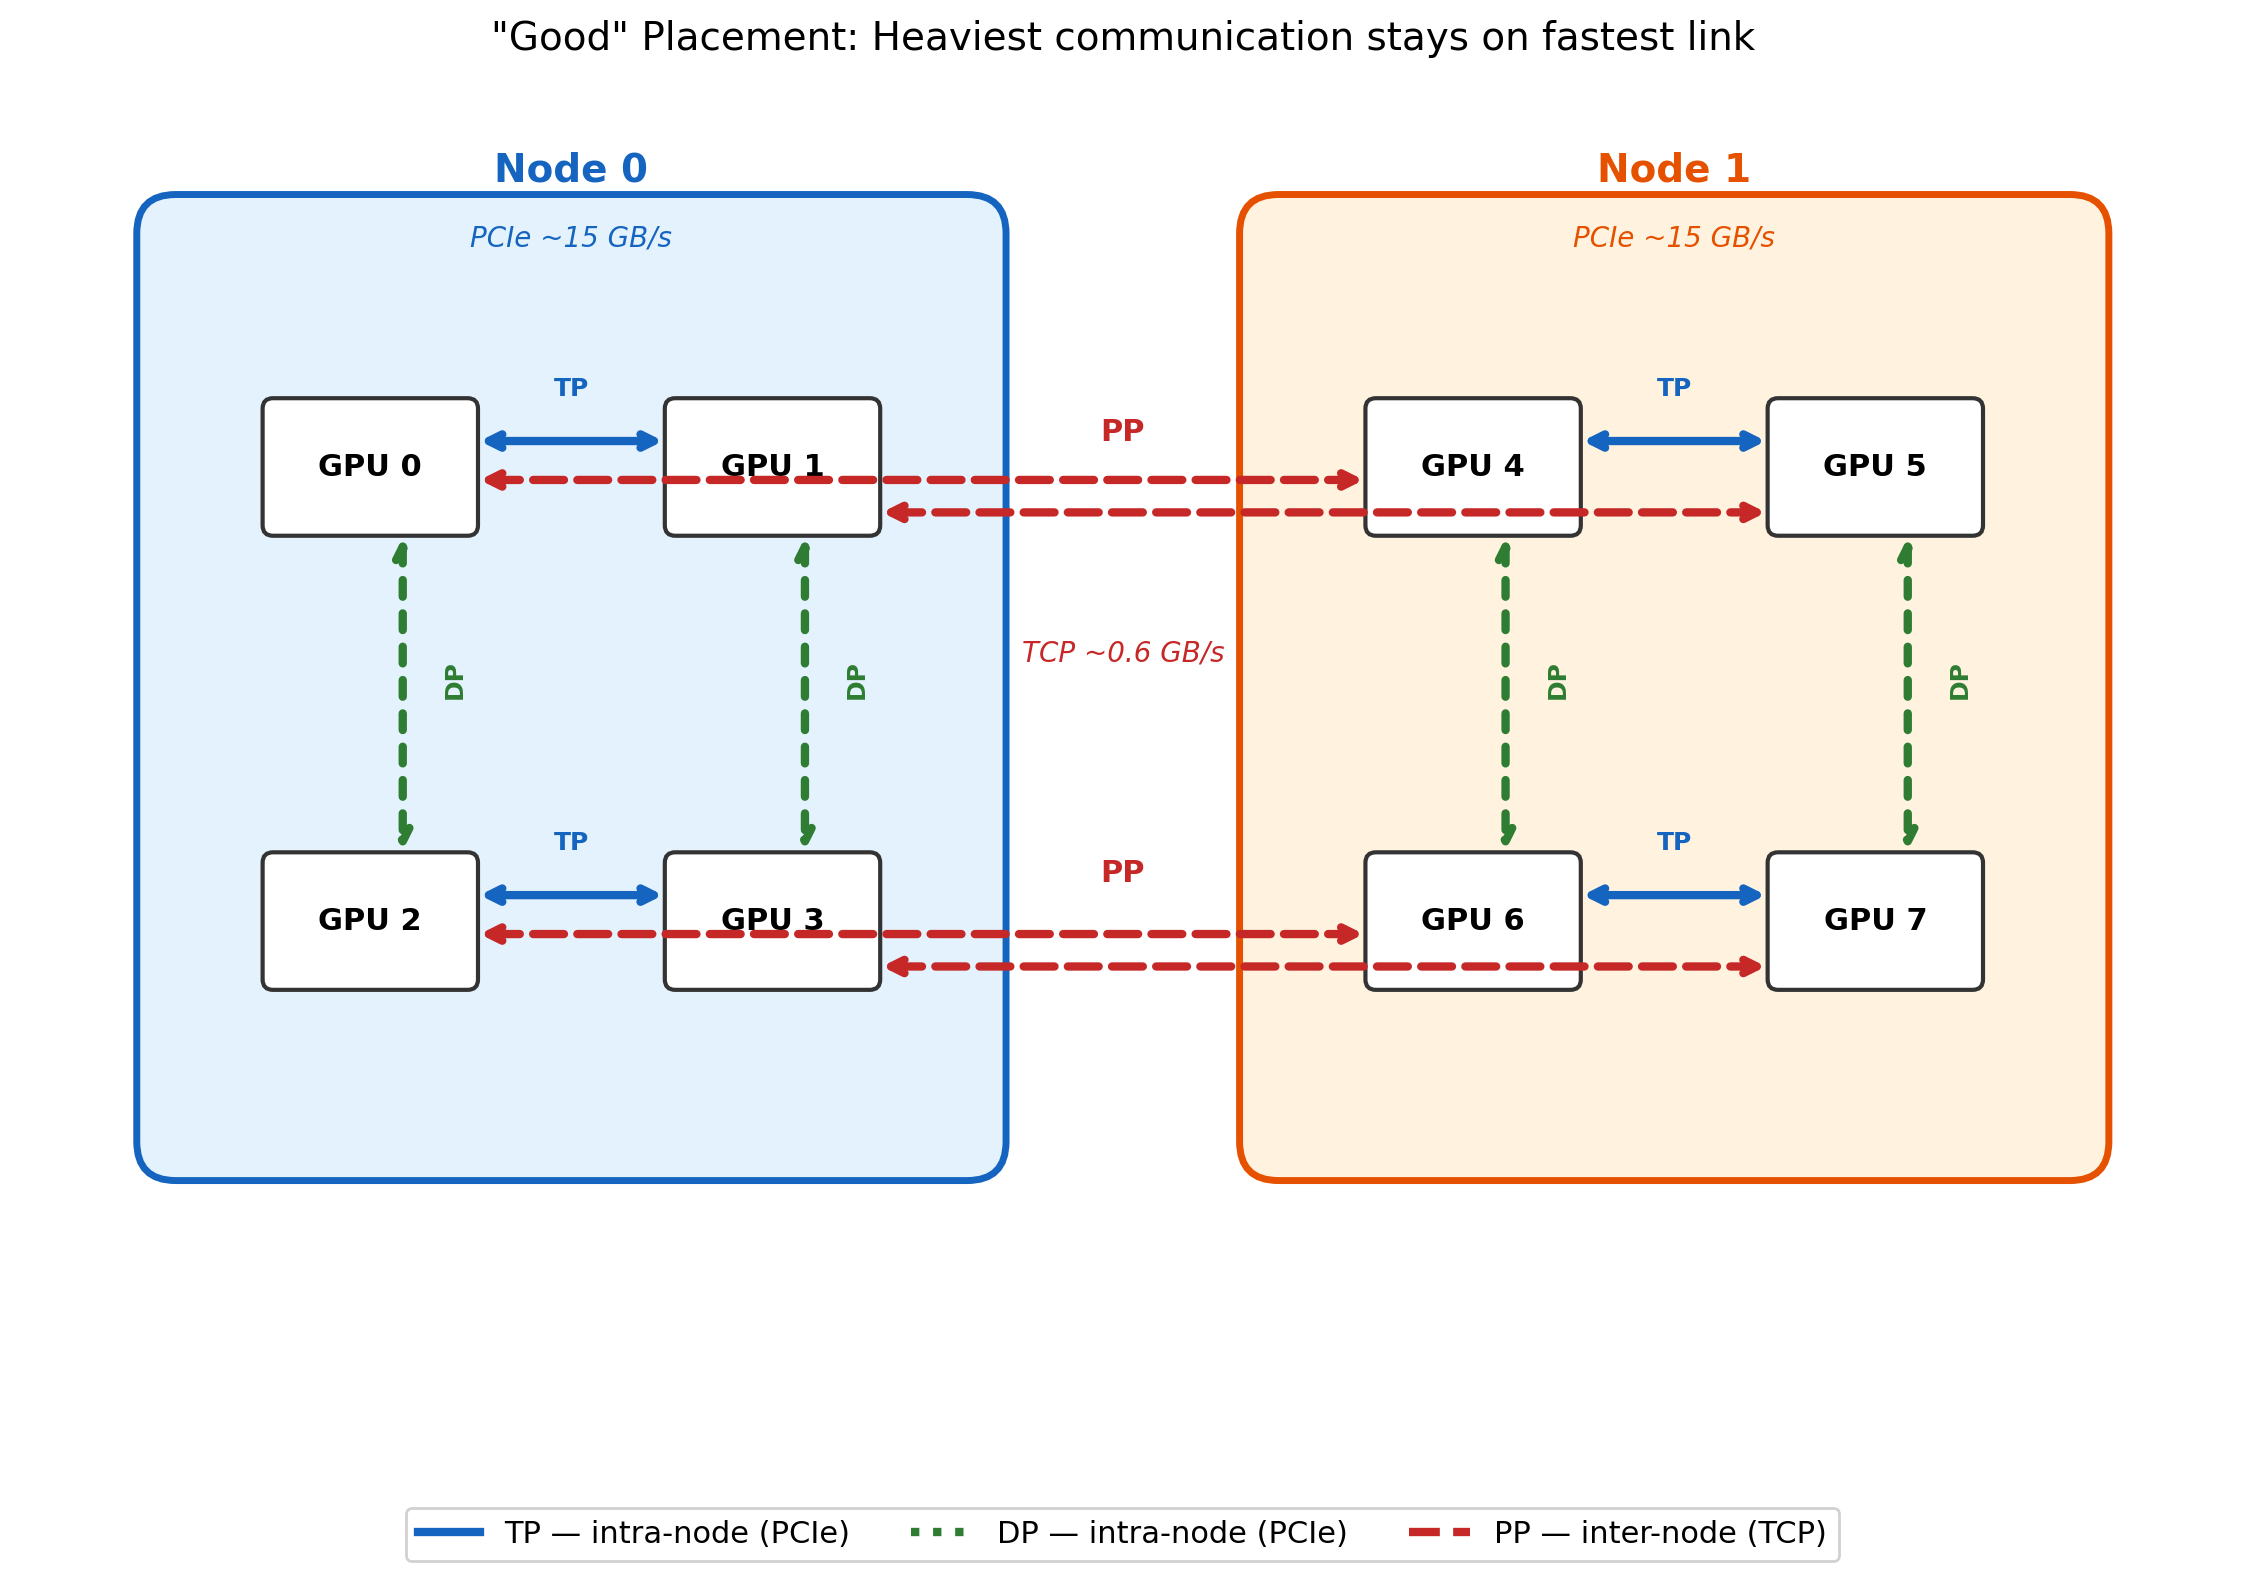
\includegraphics[width=0.68\textwidth]{fig_ppt_comm_aware_placement.png}

  \vspace{-0.2em}
  \scriptsize
  Three configs tested: \textbf{Good} (PP inter), \textbf{TP inter-node}, \textbf{Bad} (DP inter).
\end{frame}

% --- Models Used ---
\begin{frame}{Methodology: Models Used}
  \begin{columns}[T]
  \begin{column}{0.47\textwidth}
    \centering
    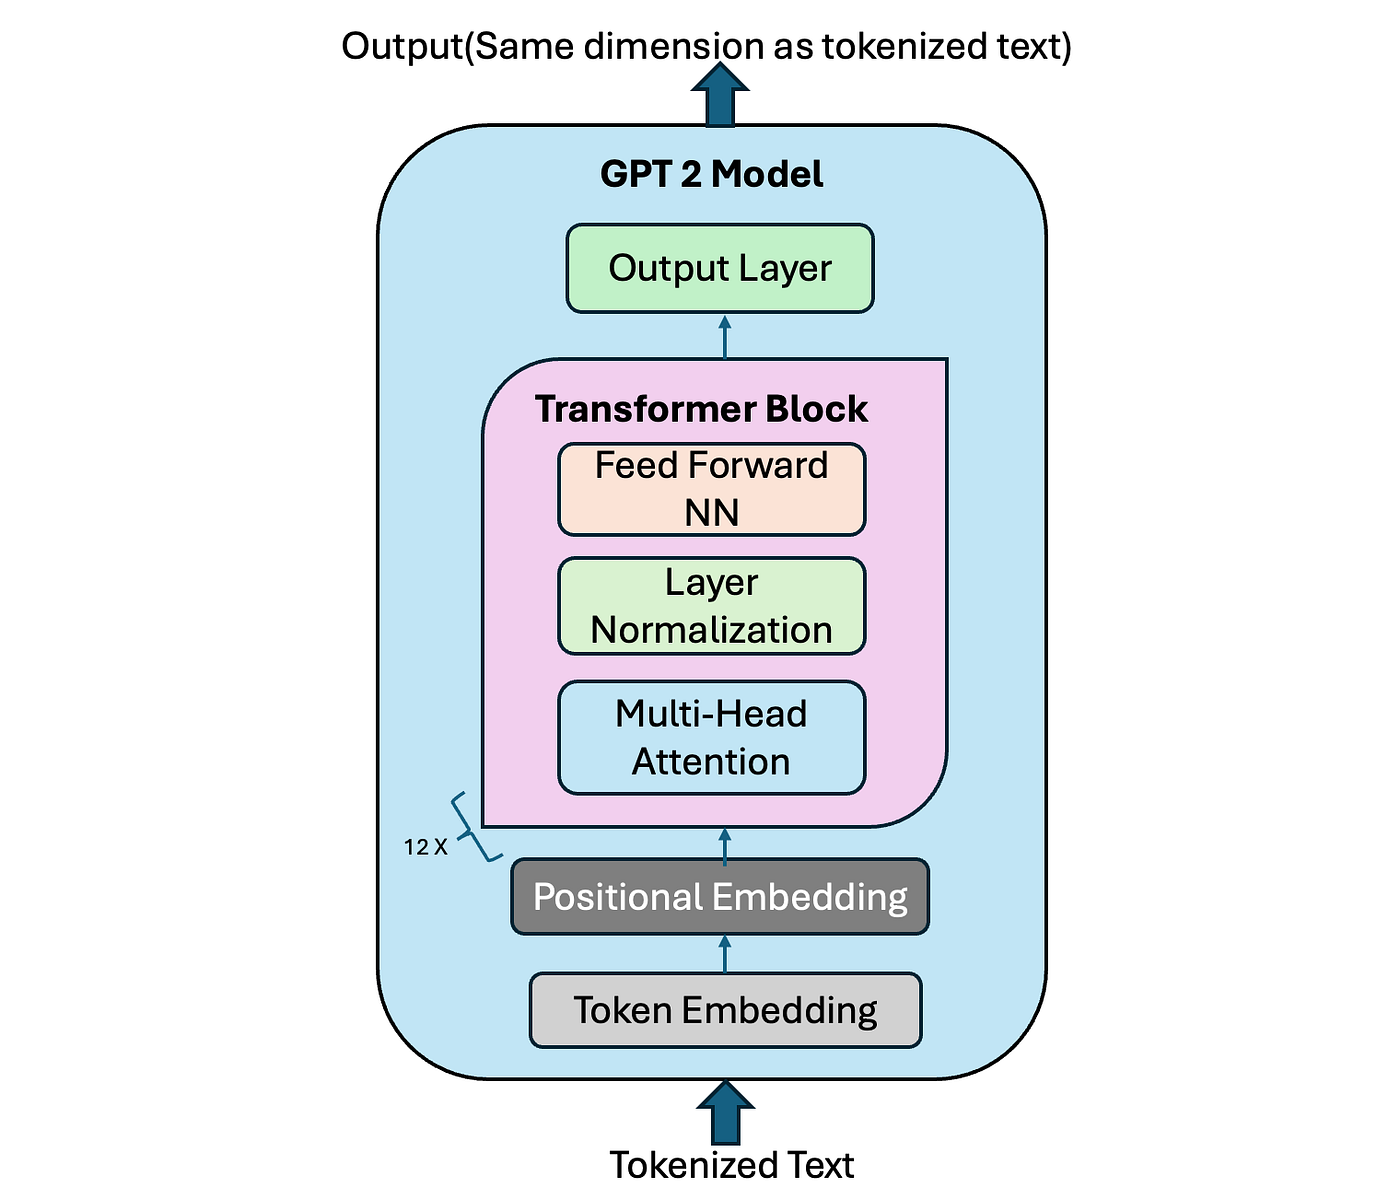
\includegraphics[width=0.75\textwidth]{GPT2.png}

    \vspace{0.3em}
    \small
    \textbf{GPT-2} (Decoder-only)\\
    Small: 117M, Medium: 354M, Large: 774M\\
    All blocks identical $\Rightarrow$ balanced pipeline
  \end{column}
  \begin{column}{0.47\textwidth}
    \centering
    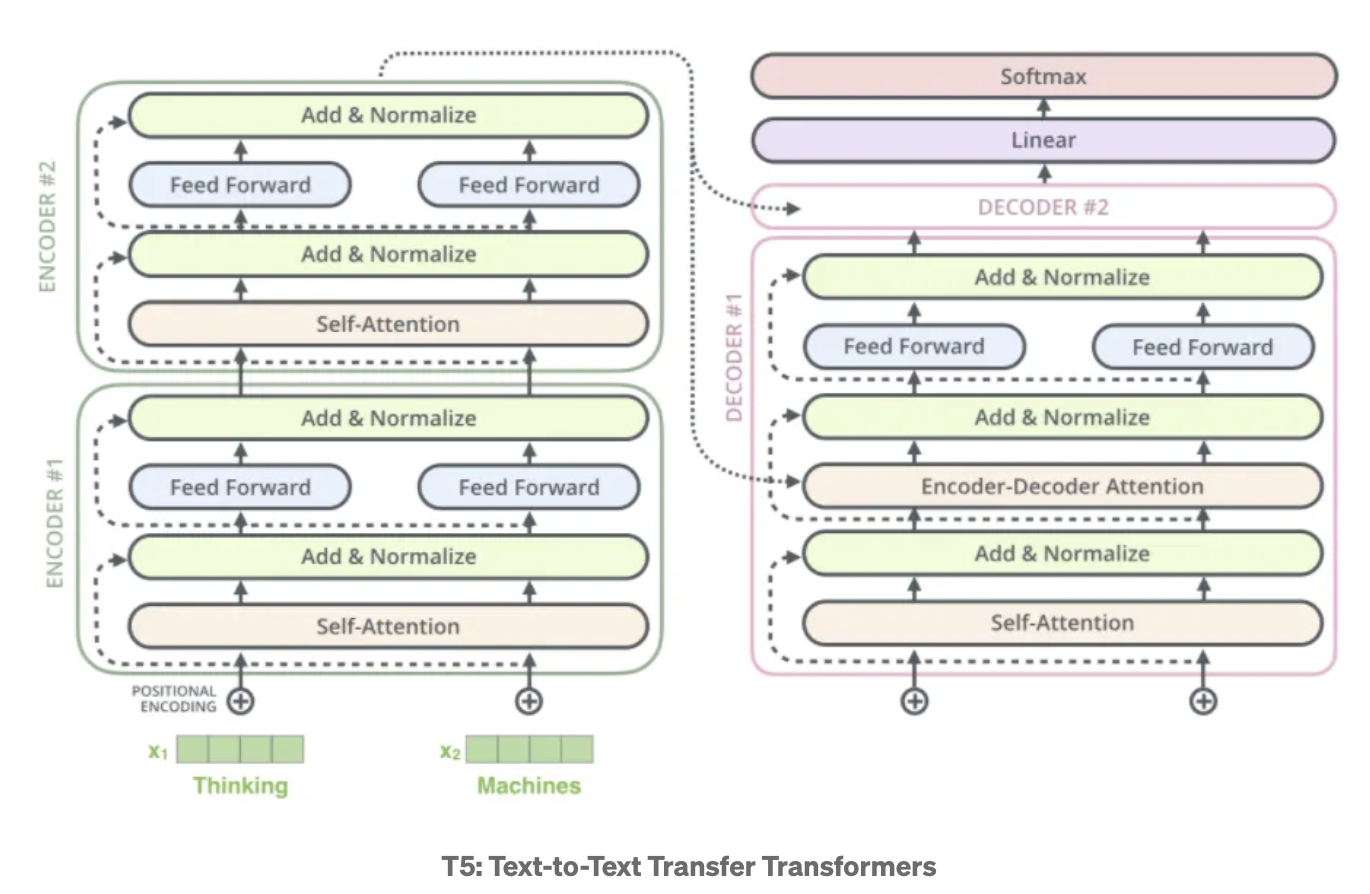
\includegraphics[width=0.85\textwidth]{T5.png}

    \vspace{0.3em}
    \small
    \textbf{T5-base} (Encoder-Decoder, 237M)\\
    Decoder has extra cross-attention sublayer\\
    Encoder lighter than decoder $\Rightarrow$ pipeline imbalance
  \end{column}
  \end{columns}
\end{frame}

% ==================================================================
% RESULTS  (Meena + Dinesh)
% ==================================================================

% --- PCIe vs TCP (Meena) ---
\begin{frame}{Results: Why Interconnect Speed Changes Everything}
  \small \textit{Setup: 4 GPUs on 1 node (PCIe) vs.\ 4 GPUs across 4 nodes (TCP) --- GPT-2 Medium (354M)}

  \vspace{-0.3em}
  \centering
  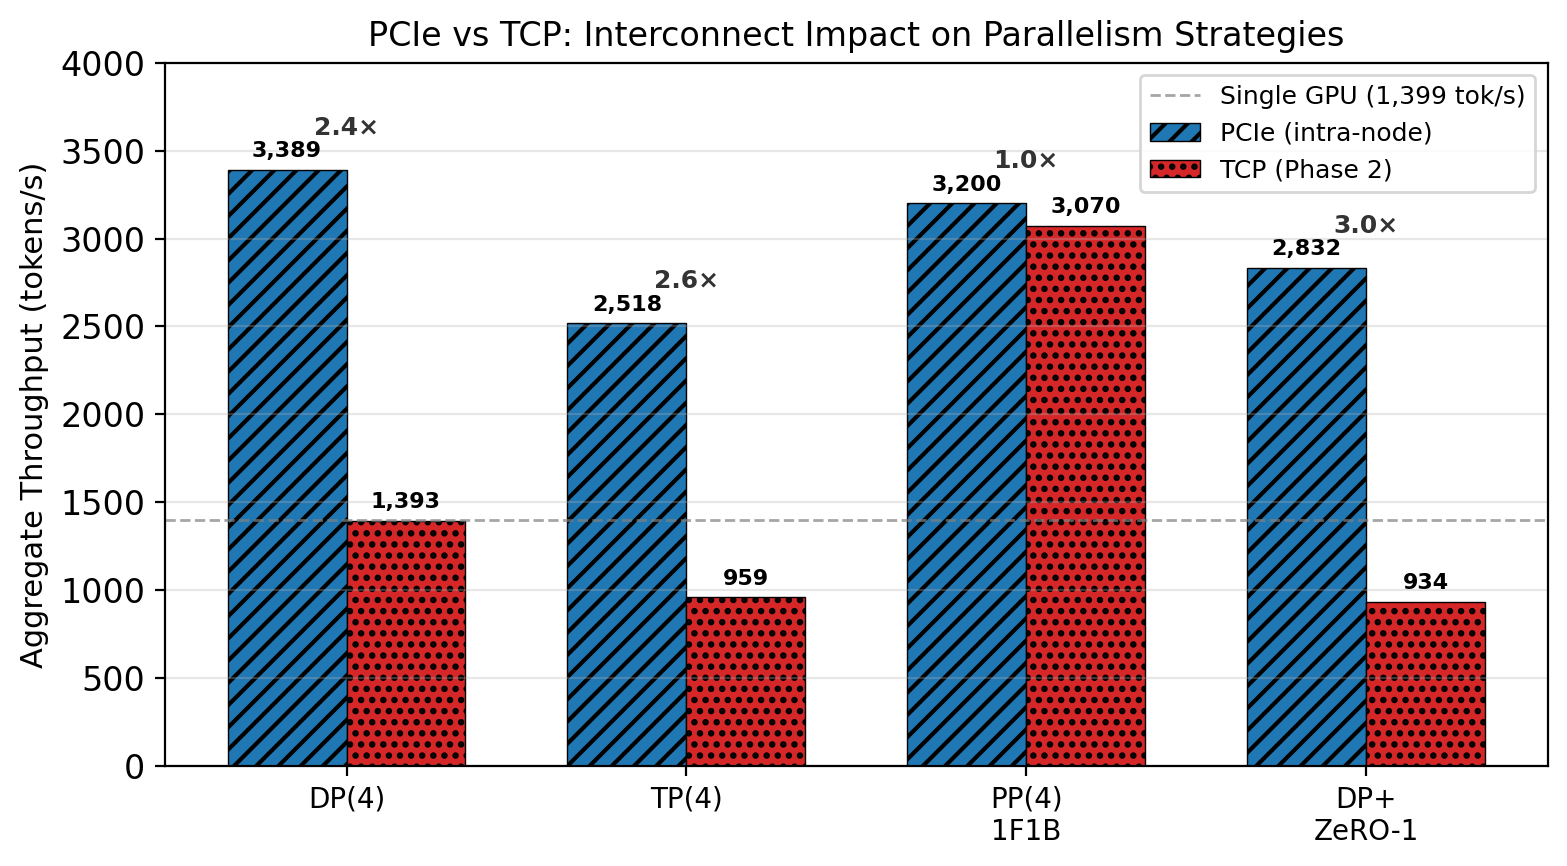
\includegraphics[width=0.70\textwidth]{fig_phase3_pcie_vs_tcp.png}

  \vspace{0.1em}
  \small
  DP, TP, ZeRO: \textbf{2.4--3$\times$} speedup on PCIe \hspace{1em}|\hspace{1em}
  PP: only \textbf{1.04$\times$} (sends small activation tensors)\\[0.3em]
  $\Rightarrow$ PP can tolerate the slow link; DP and TP cannot.
\end{frame}

% --- GPT-2 Hybrid Placement (Meena) ---
\begin{frame}{Results: GPT-2 Hybrid Placement (3 Configurations)}
  \small \textit{Setup: dp=2, pp=2, tp=2 on 8 GPUs across 2 nodes --- GPT-2 Medium (354M)}

  \begin{columns}
  \begin{column}{0.55\textwidth}
    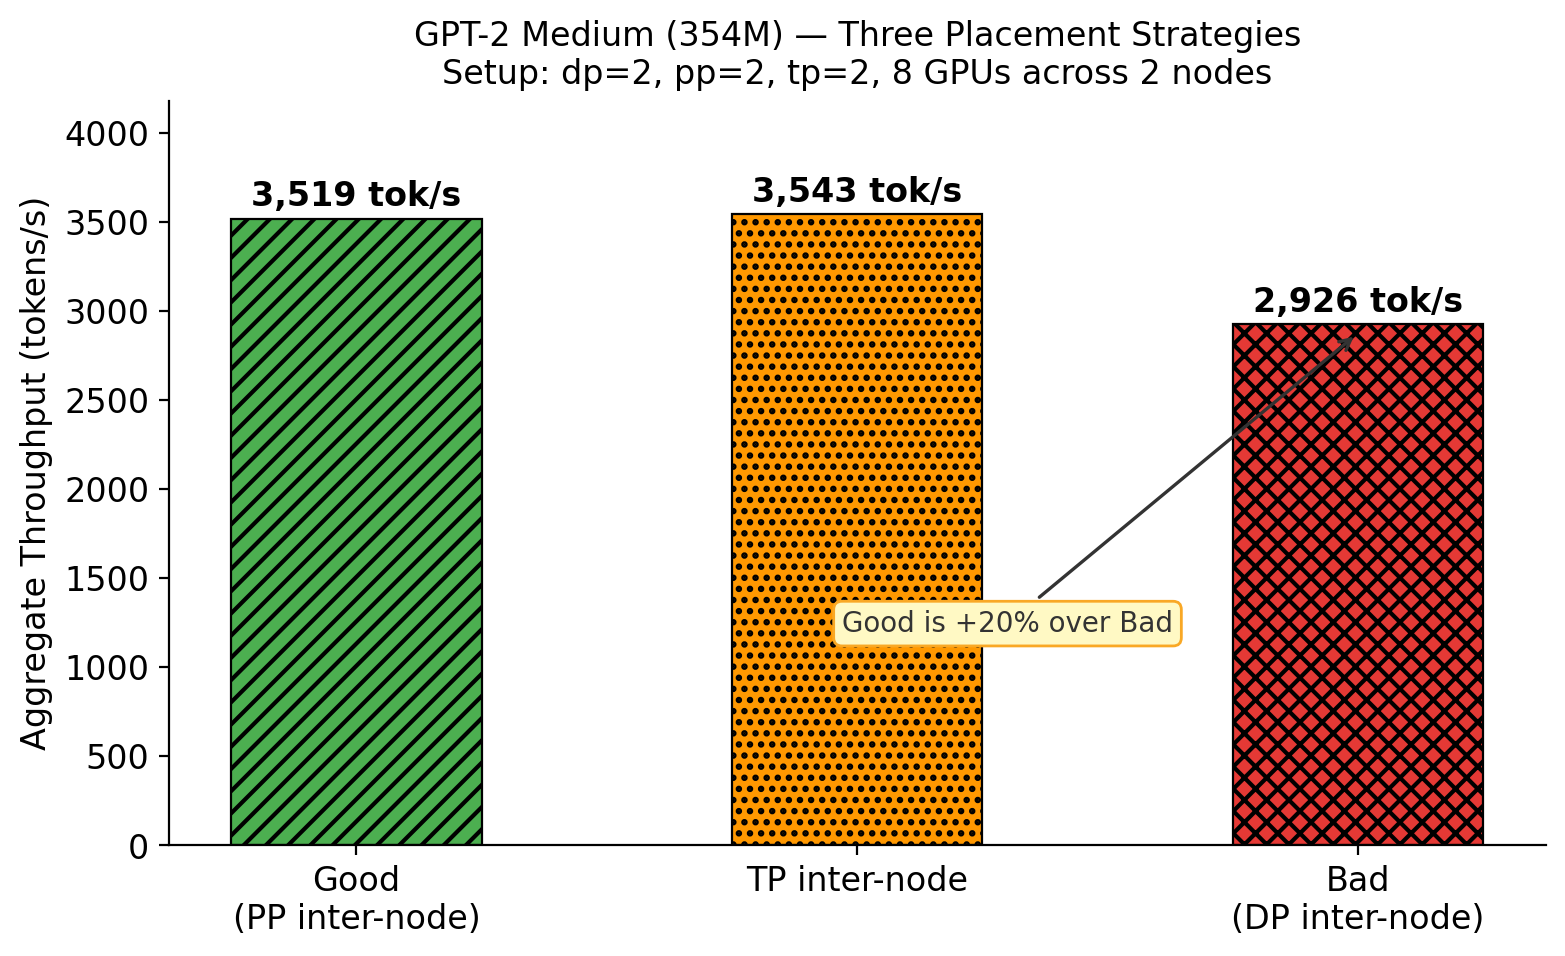
\includegraphics[width=\textwidth]{fig_ppt_gpt2_three_way.png}
  \end{column}
  \begin{column}{0.42\textwidth}
    \small
    \textbf{Good} and \textbf{TP inter-node} are almost identical ($\sim$3,500 tok/s).

    \vspace{0.3em}
    \textbf{Bad} (DP inter-node) drops to 2,926 --- a \textbf{20\% penalty}.

    \vspace{0.5em}
    With ZeRO-1 added, the gap widens further (Good 3,044 vs Bad 2,416 = \textbf{$+$26\%}).

    \vspace{0.5em}
    The bottleneck is not TP (small messages at TP=2), but \textbf{DP gradient sync} ($\sim$1.4 GB transferred in one shot).
  \end{column}
  \end{columns}
\end{frame}

% --- T5 Hybrid Placement (Dinesh) ---
\begin{frame}{Results: T5-base Hybrid Placement (3 Configurations)}
  \small \textit{Setup: dp=2, pp=2, tp=2 on 8 GPUs across 2 nodes --- T5-base (237M)}

  \begin{columns}
  \begin{column}{0.55\textwidth}
    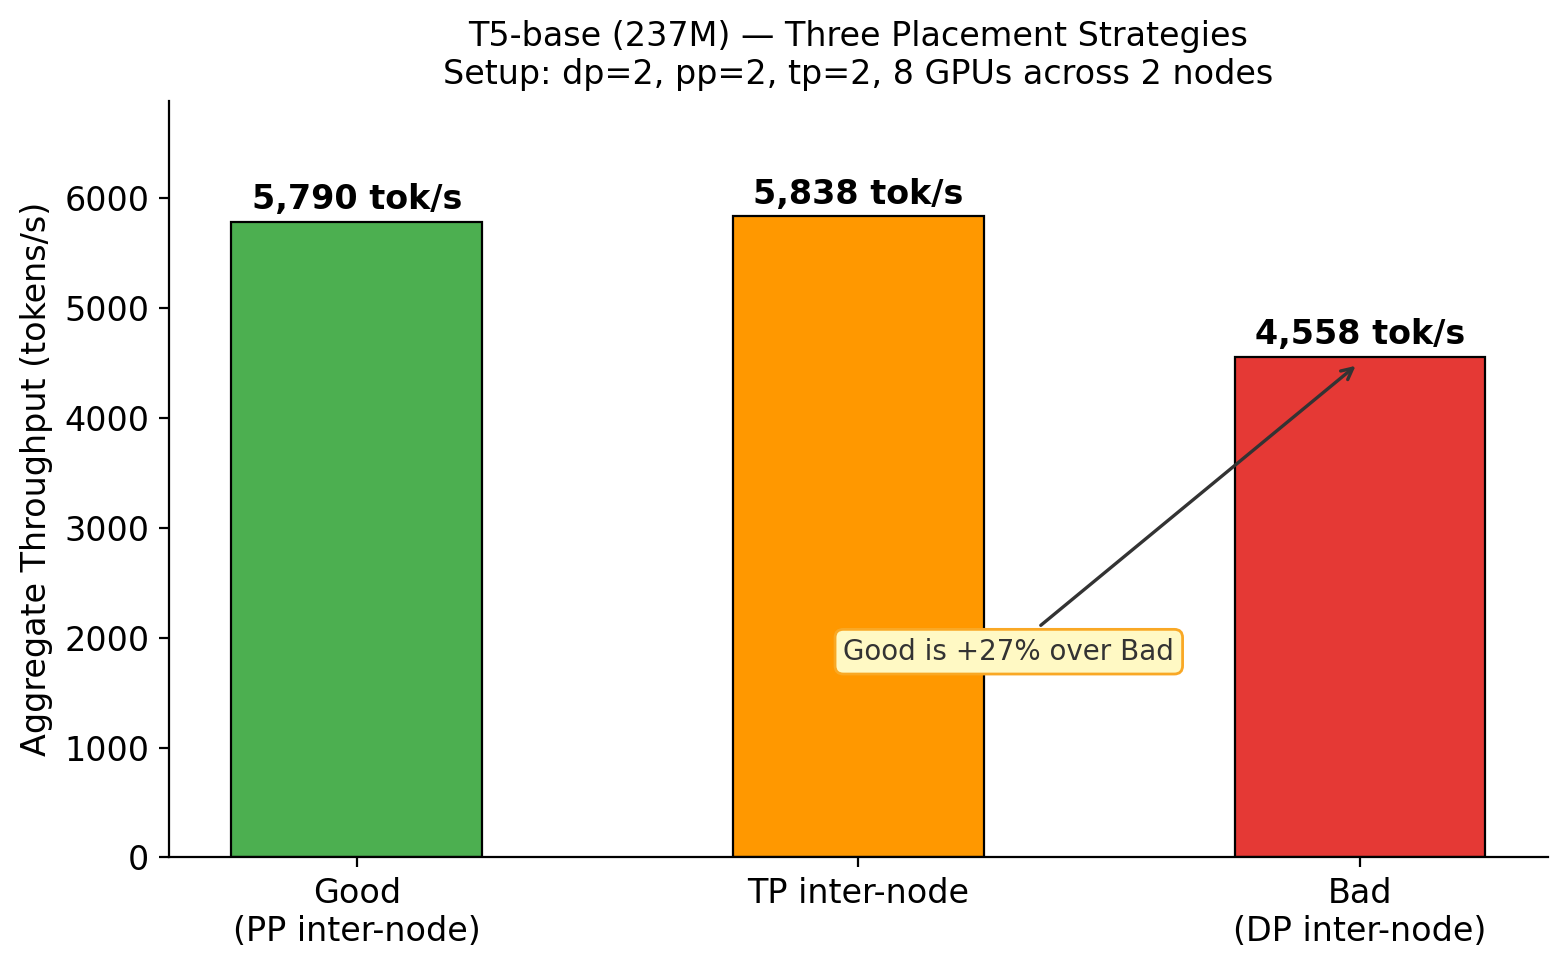
\includegraphics[width=\textwidth]{fig_ppt_t5_three_way.png}
  \end{column}
  \begin{column}{0.42\textwidth}
    \small
    Same pattern as GPT-2: Good $\approx$ TP-inter, Bad is worst.

    \vspace{0.3em}
    But the penalty is \textbf{larger for T5: +27\%} (vs +20\% for GPT-2).

    \vspace{0.5em}
    Why? T5 has more communication per step (60 vs 48 TP all-reduces due to cross-attention) and faster compute, so it is more \textbf{communication-bound}.

    \vspace{0.3em}
    Any slow-link overhead hits harder when communication is already a large fraction of step time.
  \end{column}
  \end{columns}
\end{frame}

% --- Multi-Model Scaling (Dinesh) ---
\begin{frame}{Results: Does Hybrid Scaling Depend on Architecture?}
  \small \textit{Setup: dp=2, pp=2, tp=2, good placement --- single GPU vs 8-GPU hybrid}

  \begin{columns}
  \begin{column}{0.55\textwidth}
    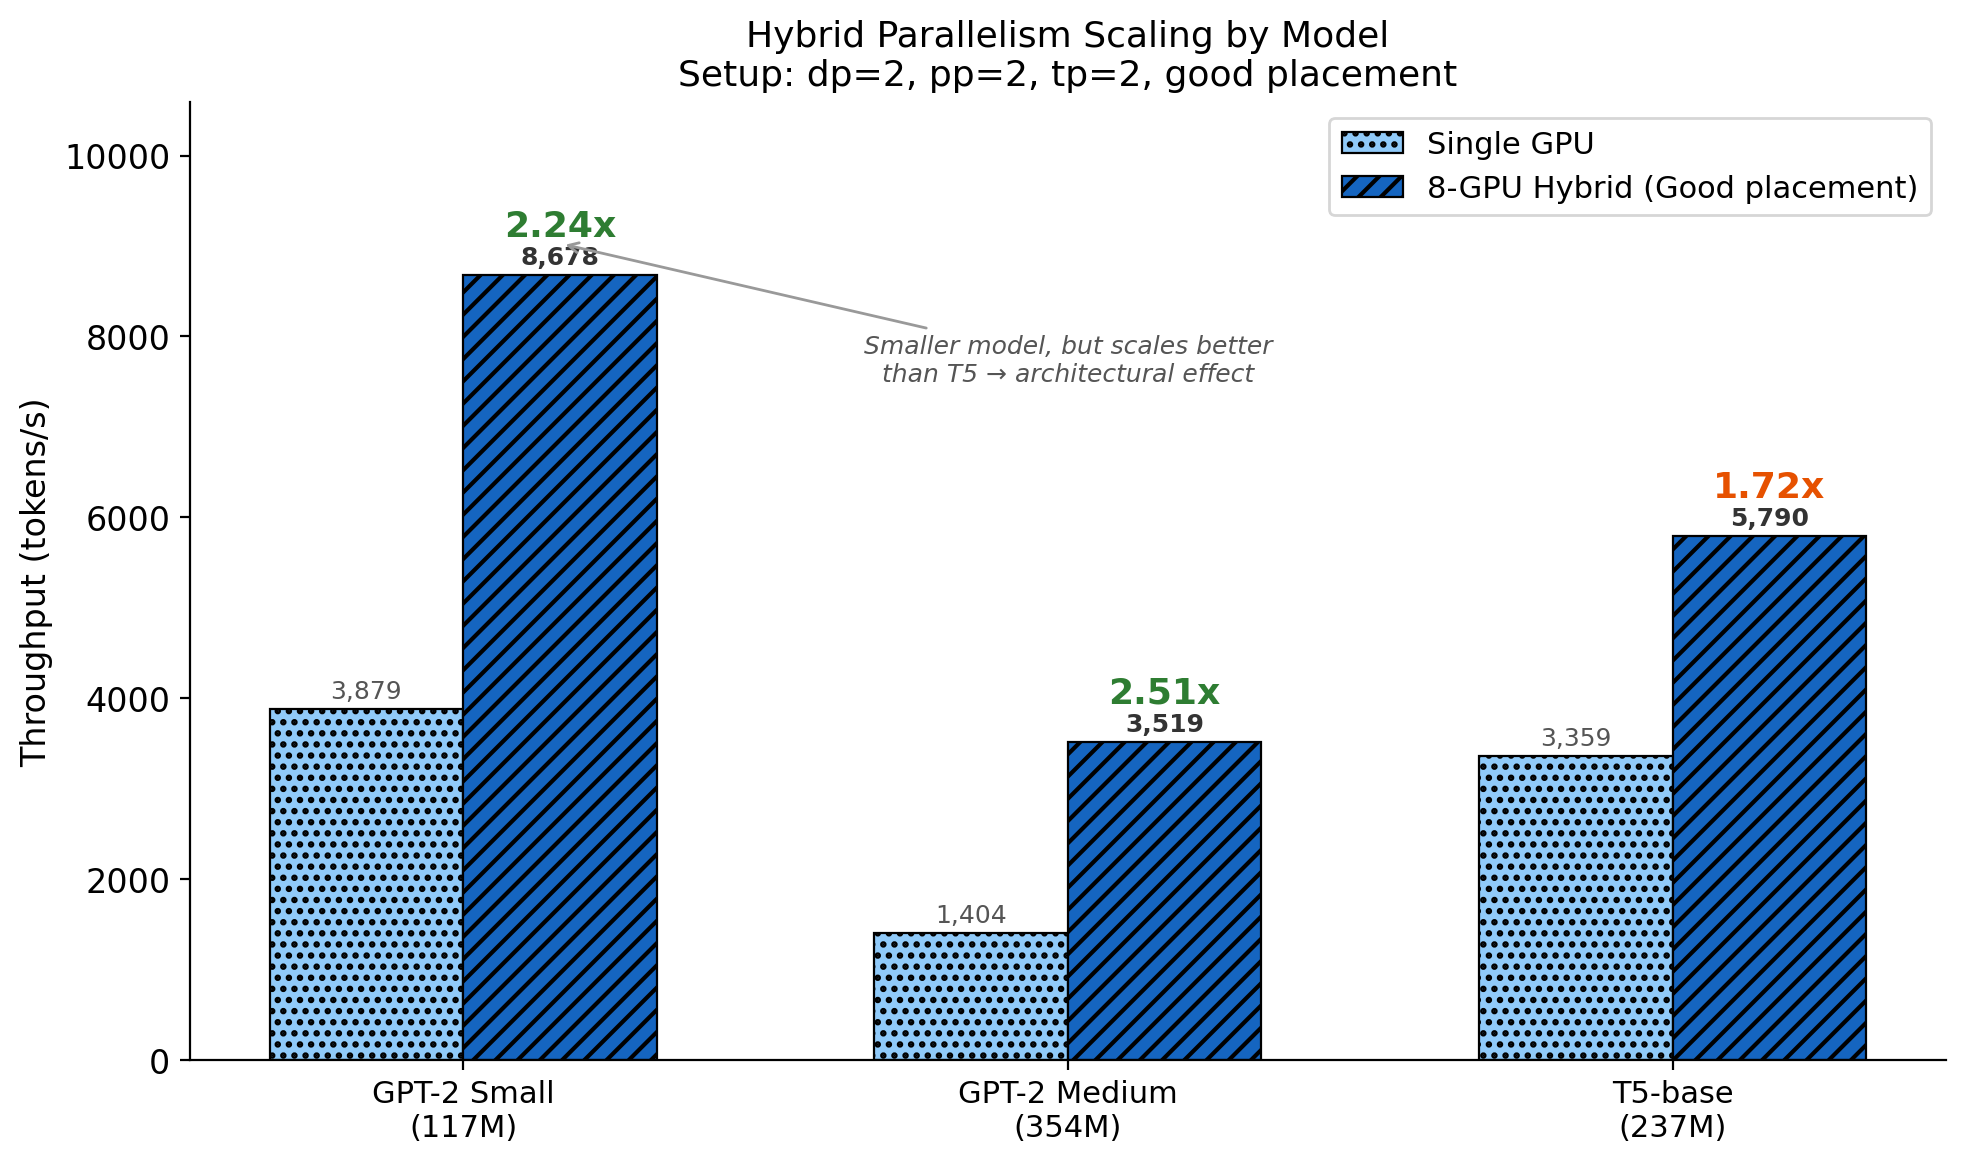
\includegraphics[width=\textwidth]{fig_ppt_model_scaling.png}
  \end{column}
  \begin{column}{0.42\textwidth}
    \small
    GPT-2 models: \textbf{2.2--2.5$\times$} speedup.

    T5-base: only \textbf{1.72$\times$} speedup.

    \vspace{0.5em}
    GPT-2 Small (117M) is \textit{smaller} than T5 (237M) but scales \textit{better}.

    \vspace{0.3em}
    $\Rightarrow$ The gap is architectural:

    \vspace{0.2em}
    \textbf{1. Pipeline imbalance}\\
    \quad GPT-2: 4.07 vs 4.08 GB\\
    \quad T5: 2.51 vs 3.87 GB (54\%)

    \vspace{0.2em}
    \textbf{2. Extra TP all-reduces}\\
    \quad GPT-2 Med: 48 per fwd\\
    \quad T5-base: 60 per fwd (+25\%)
  \end{column}
  \end{columns}
\end{frame}

% ==================================================================
% KEY FINDINGS  (Dinesh)
% ==================================================================

\begin{frame}{Key Findings}
  \begin{enumerate}
    \item \textbf{Placement delivers 17--27\% throughput gain}\\
    Keeping bandwidth-heavy axes (DP, TP) on the fast intra-node link consistently outperforms the reverse, across all models.

    \vspace{0.3em}
    \item \textbf{DP overtakes TP as the placement bottleneck at low TP degrees}\\
    Standard expectation: TP is most sensitive (all-reduce every layer).
    At TP=2, individual TP messages are small (KB--MB) and TCP handles them fine.
    DP gradient sync ($\sim$1 GB+) saturates the slow link.
    At higher TP degrees (4, 8), TP would become the bottleneck again.

    \vspace{0.3em}
    \item \textbf{Encoder-decoder models amplify the placement penalty}\\
    T5 sees +27\% gain from good placement vs +20\% for GPT-2. T5's extra cross-attention all-reduces make it more communication-bound, so slow-link overhead hits harder.

    \vspace{0.3em}
    \item \textbf{Symmetric vs asymmetric architectures: 30--46\% scaling gap}\\
    GPT-2's identical blocks give balanced pipeline stages and fewer all-reduces.
    T5's encoder-decoder split creates 54\% memory imbalance and 25\% more TP communication.
  \end{enumerate}
\end{frame}

% ==================================================================
% SUMMARY  (Nadhiya)
% ==================================================================

\begin{frame}{Summary}
  \begin{columns}[T]
  \begin{column}{0.55\textwidth}
    \textbf{What we built:}
    \begin{itemize}
      \item Four parallelism strategies from scratch
      \item Unified 3D hybrid plugin (DP$\times$PP$\times$TP)
      \item T5-base encoder-decoder implementation
    \end{itemize}

    \vspace{0.5em}
    \textbf{What we showed:}
    \begin{itemize}
      \item On a heterogeneous cluster, mapping axes to network tiers based on their communication volume gives 17--27\% throughput gains
      \item DP is the most sensitive axis at low parallelism degrees
      \item Hybrid parallelism benefits depend on model architecture --- symmetric GPT-2 scales 30--46\% better than asymmetric T5
    \end{itemize}
  \end{column}
  \begin{column}{0.42\textwidth}
    \centering
    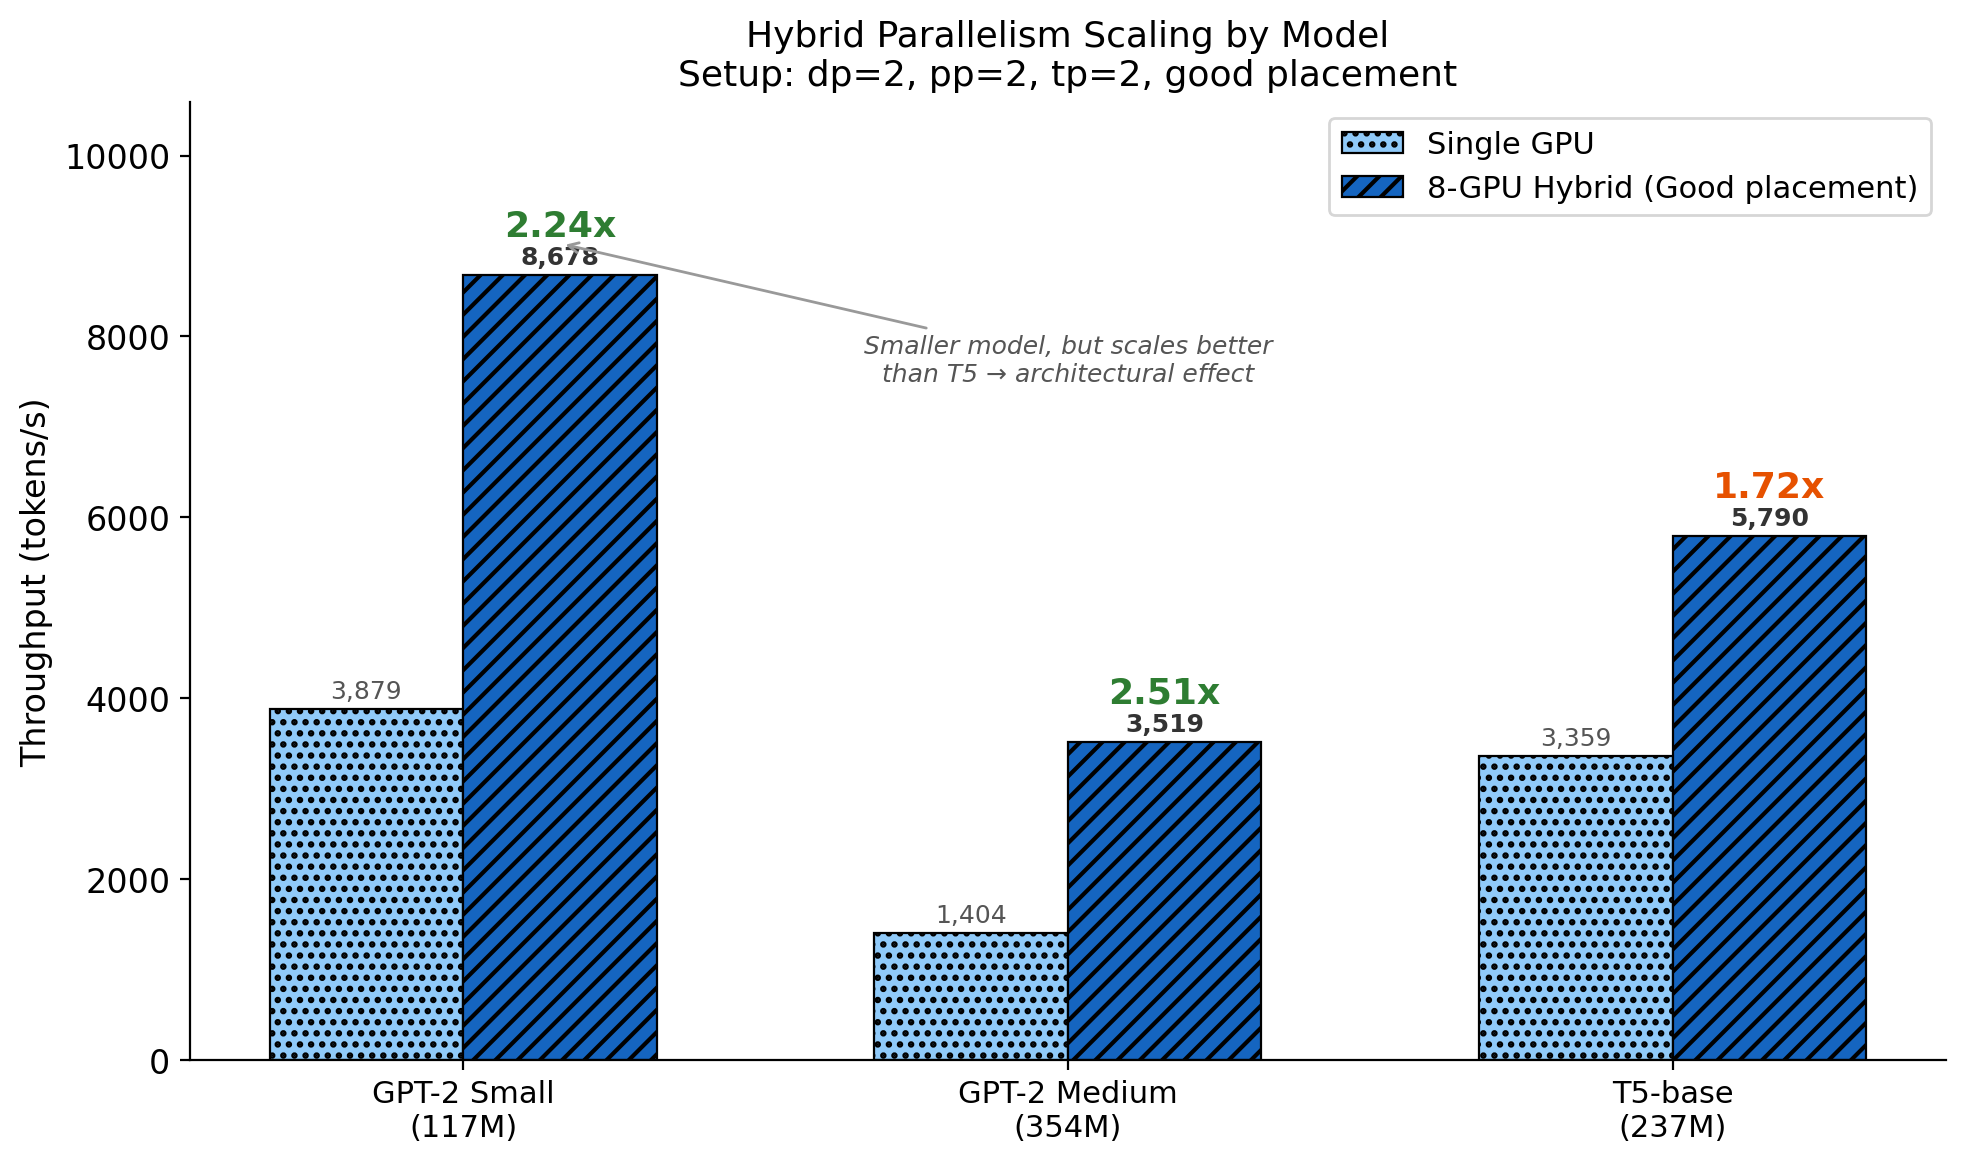
\includegraphics[width=\textwidth]{fig_ppt_model_scaling.png}

    \vspace{0.3em}
    \small
    Same hardware, same config ---\\
    architecture determines the scaling.
  \end{column}
  \end{columns}
\end{frame}

% ======== QUESTIONS ========
\begin{frame}
  \centering
  \vspace{2cm}
  {\Huge\bfseries Questions?}
  \vspace{1cm}

  {\large Dinesh Chand \quad Goutham P \quad Meena Chidambaram \quad Nadhiya R S}

  \vspace{0.3em}
  {\small MTech-AI, IISc Bangalore}
\end{frame}

\end{document}
